% Options for packages loaded elsewhere
\PassOptionsToPackage{unicode}{hyperref}
\PassOptionsToPackage{hyphens}{url}
%
\documentclass[
]{article}
\usepackage{amsmath,amssymb}
\usepackage{lmodern}
\usepackage{iftex}
\ifPDFTeX
  \usepackage[T1]{fontenc}
  \usepackage[utf8]{inputenc}
  \usepackage{textcomp} % provide euro and other symbols
\else % if luatex or xetex
  \usepackage{unicode-math}
  \defaultfontfeatures{Scale=MatchLowercase}
  \defaultfontfeatures[\rmfamily]{Ligatures=TeX,Scale=1}
\fi
% Use upquote if available, for straight quotes in verbatim environments
\IfFileExists{upquote.sty}{\usepackage{upquote}}{}
\IfFileExists{microtype.sty}{% use microtype if available
  \usepackage[]{microtype}
  \UseMicrotypeSet[protrusion]{basicmath} % disable protrusion for tt fonts
}{}
\makeatletter
\@ifundefined{KOMAClassName}{% if non-KOMA class
  \IfFileExists{parskip.sty}{%
    \usepackage{parskip}
  }{% else
    \setlength{\parindent}{0pt}
    \setlength{\parskip}{6pt plus 2pt minus 1pt}}
}{% if KOMA class
  \KOMAoptions{parskip=half}}
\makeatother
\usepackage{xcolor}
\IfFileExists{xurl.sty}{\usepackage{xurl}}{} % add URL line breaks if available
\IfFileExists{bookmark.sty}{\usepackage{bookmark}}{\usepackage{hyperref}}
\hypersetup{
  pdftitle={Exploring the seasonal variation in electric vehicle charging in New Zealand},
  pdfauthor={Pablo Paulsen},
  hidelinks,
  pdfcreator={LaTeX via pandoc}}
\urlstyle{same} % disable monospaced font for URLs
\usepackage[margin=1in]{geometry}
\usepackage{graphicx}
\makeatletter
\def\maxwidth{\ifdim\Gin@nat@width>\linewidth\linewidth\else\Gin@nat@width\fi}
\def\maxheight{\ifdim\Gin@nat@height>\textheight\textheight\else\Gin@nat@height\fi}
\makeatother
% Scale images if necessary, so that they will not overflow the page
% margins by default, and it is still possible to overwrite the defaults
% using explicit options in \includegraphics[width, height, ...]{}
\setkeys{Gin}{width=\maxwidth,height=\maxheight,keepaspectratio}
% Set default figure placement to htbp
\makeatletter
\def\fps@figure{htbp}
\makeatother
\setlength{\emergencystretch}{3em} % prevent overfull lines
\providecommand{\tightlist}{%
  \setlength{\itemsep}{0pt}\setlength{\parskip}{0pt}}
\setcounter{secnumdepth}{-\maxdimen} % remove section numbering
\usepackage{float}
\floatplacement{figure}{H}
\usepackage{comment}
\ifLuaTeX
  \usepackage{selnolig}  % disable illegal ligatures
\fi

\title{Exploring the seasonal variation in electric vehicle charging in
New Zealand}
\author{Pablo Paulsen}
\date{02/18/2022}

\begin{document}
\maketitle

\hypertarget{data-exploration}{%
\subsection{Data Exploration}\label{data-exploration}}

Distance traveled and vehicle efficiency (km/kWh) by month, as well as
the region of the vehicle was collected from the on-board computers of
1259 vehicles between 2017 and 2021 as part of the `Flip the Fleet'
project.

A monthly weighted average was calculated for the whole of New Zealand
and then for each region of NZ. The monthly averages were weighted using
the distance traveled to give more weighting to vehicles with higher km
traveled in that month. this was done using the formula
\[\bar{x} = \frac{\sum_{i}^{n} (d_i\times x_i)}{\left(\sum_{i}^{n} d_i\right)\times n}\]

Power consumption (Wh/km) was calculated using the efficiency (km/kWh).
This will be used instead of efficiency in the modeling for reasons that
will become apparent later in the analysis.

\begin{figure}
\centering
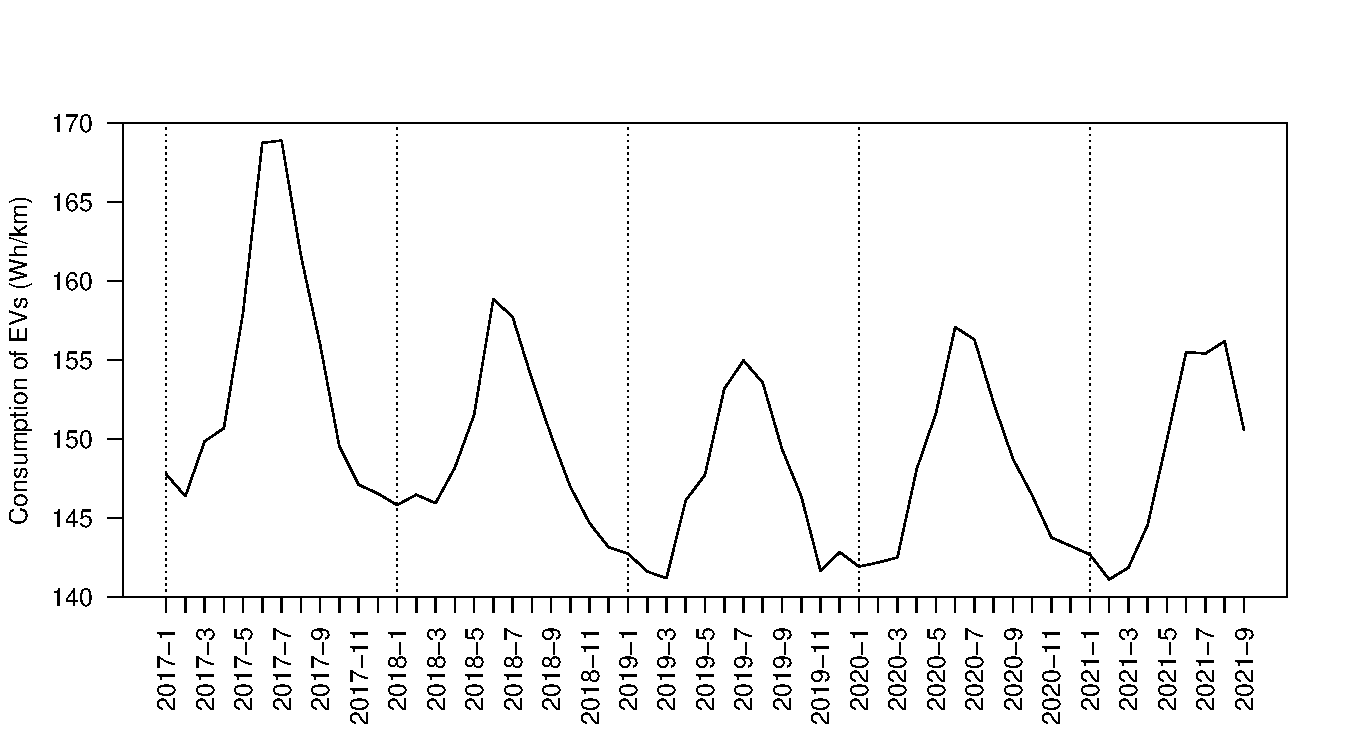
\includegraphics{final_report_files/figure-latex/eff_plot-1.pdf}
\caption{Time series of EVs weighted mean consumption using Flip the
Fleet data from all of NZ}
\end{figure}

\end{document}
